\documentclass{article}
%
\usepackage[utf8]{vietnam}
\usepackage[a4paper, top=2cm, left=2cm, right=2cm, bottom=2cm]{geometry}
\usepackage{amsmath}
\usepackage{setspace}
\usepackage{graphicx}
\usepackage{icomma}
\usepackage{scrextend}
\usepackage{siunitx}
\usepackage{fancyhdr}
\usepackage{subfigure}

%
\changefontsizes{13pt}
\pagestyle{fancy}
\fancyhf{}
\rhead{Nguyễn Minh Đăng - 20230022}
\fancyfoot[C]{\thepage}
\changefontsizes{13pt}

\begin{document}
\onehalfspacing
{
   \setlength{\topmargin}{-0.5cm}
\begin{titlepage}
  \begin{center}
    \centerline{
\includegraphics[height=42mm]{logo}}

    
   \vspace{1cm}

        {\large Trường Đại học Khoa học Tự nhiên}\\[1em]
        {\large Đại học Quốc gia Thành phố Hồ Chí Minh}
    
        \vspace{1.2cm}
    \centerline{\hbox to 13cm{\hrulefill}}
    \vspace{0.3cm}
    \Large  {{Thực Tập Chuyên Đề 1 }}
    \centerline{\hbox to 13cm{\hrulefill}}
    
    \vspace{1.2cm}
    \Large {Bài 8: Xây Dựng Đường Chuẩn Năng Lượng \\ Của Một Nguồn Phóng Xạ}\\ 
   
   \vspace{3cm}
            \large Người hướng dẫn: Thầy Châu Thành Tài \\ 
            \large Sinh viên: Nguyễn Minh Đăng - 20230022
    
    \vspace{4cm}
    

    
    \hbox to \textwidth{\hrulefill}
    \vspace{0.2cm}
    {\sc  17/04/2023}
    
  \end{center}
\end{titlepage}
}

\newpage
\clearpage\thispagestyle{empty}\addtocounter{page}{-1} 
\clearpage
\mbox{}
 % creates a blank space to fill the page
\newpage
%
\setcounter{section}{1}
\section*{\centering Báo Cáo Kết Quả}
\vspace{1cm}
%
\subsection{Lập bảng tương ứng với số kênh theo năng lượng trong bảng 1 được đo bằng detector}
Ta có các đỉnh năng lượng ứng với các kênh của nguồn Eu-152
\begin{table}[!ht]
    \centering
    \resizebox{\columnwidth}{!}{%
    \begin{tabular}{|c|c|c|c|c|c|c|c|c|c|c|c|}
    \hline
        Kênh & 444 & 918 & 1302 & 1562 & 1689 & 2981 & 3324 & 3697 & 4168 & 4269 & 5413 \\ \hline
        Năng lượng (KeV) & 121,78 & 244,70 & 344,28 & 411,12 & 443,97 & 778,90 & 867,38 & 964,08 & 1085,84 & 1112,08 & 1408,01 \\ \hline
    \end{tabular}
    }
\end{table}
\vspace{0.25cm}
%
\subsection{Xác định đường chuẩn năng lượng bằng phương pháp bình phương tối thiểu và so sánh với hệ số a và b trong chương trình Genie và chương trình Excel}
Phương trình chuẩn năng lượng có dạng
\begin{align*}
	E \ [KeV] = a.ch + b
\end{align*}
Từ đây ta có
\begin{align*}
	& v_i = a.ch + b - E \\
	& S = \sum_{i=1}^{n} v_i^2= \sum_{i=1}^{n}\Big[a.ch + b - E\Big]^2 \\
	& S = \sum_{i=1}^{n}\Big[a^2.ch^2 + b^2 + E^2 + 2a.ch.b - 2a.ch.E - 2b.E \Big]
\end{align*}
Để tìm được thông số $a_r$ thì ta đặt cho $S$ là cực tiểu:
\begin{align*}
	\rightarrow \frac{\partial S}{\partial a_r} = 0
\end{align*}
Từ đây ta có:
\begin{itemize} 
	\item $\begin{aligned}
				 \frac{\partial S}{\partial a} = 2a.ch^2 + 2ch.b - 2ch.E = 0
\end{aligned}$
\end{itemize}
\begin{align}
	\rightarrow a \sum{ch^2} + b\sum{ch} = \sum{ch.E}
\end{align}
\begin{itemize} 
	\item $\begin{aligned}
				 \frac{\partial S}{\partial b} = 2b + 2a.ch - 2E = 0
\end{aligned}$
\end{itemize}
\begin{align}
	\rightarrow a \sum{ch} + b.n =  \sum{E}
\end{align}
Từ (1) và (2) ta có hệ phương trình
\begin{align}
	\begin{cases}
	a \sum{ch^2} + b\sum{ch} =  \sum{ch.E} \\ 
	a \sum{ch} + n.b =  \sum{E} 
	\end{cases}
\end{align}
Từ đây ta có các số
\begin{align*}
	& \sum{ch^2} = 106527929; \ \quad \sum{ch} = 29767 \\
	& \sum{ch.E} = 27783055,68; \ \quad \sum{E} = 7782,13
\end{align*}
Từ đây ta có hệ phương trình
\begin{align*}
	\begin{cases}
	106527929.a + 29767.b = 27783055,68 \\ 
	29767.a + 11b =  7782,13
	\end{cases}
	\rightarrow
	\begin{cases}
	a = 0,26 \\
	b = 6,99
	\end{cases}
\end{align*}
Từ đây ta có phương trình tuyến tính
\begin{align}
	E \ [KeV] = 0,26.ch + 6,99
\end{align}
Phương trình chuẩn năng lượng từ Genie và Excel
\begin{figure}[ht]
  \centering
  \subfigure[Phương trình chuẩn của Genie 2K]{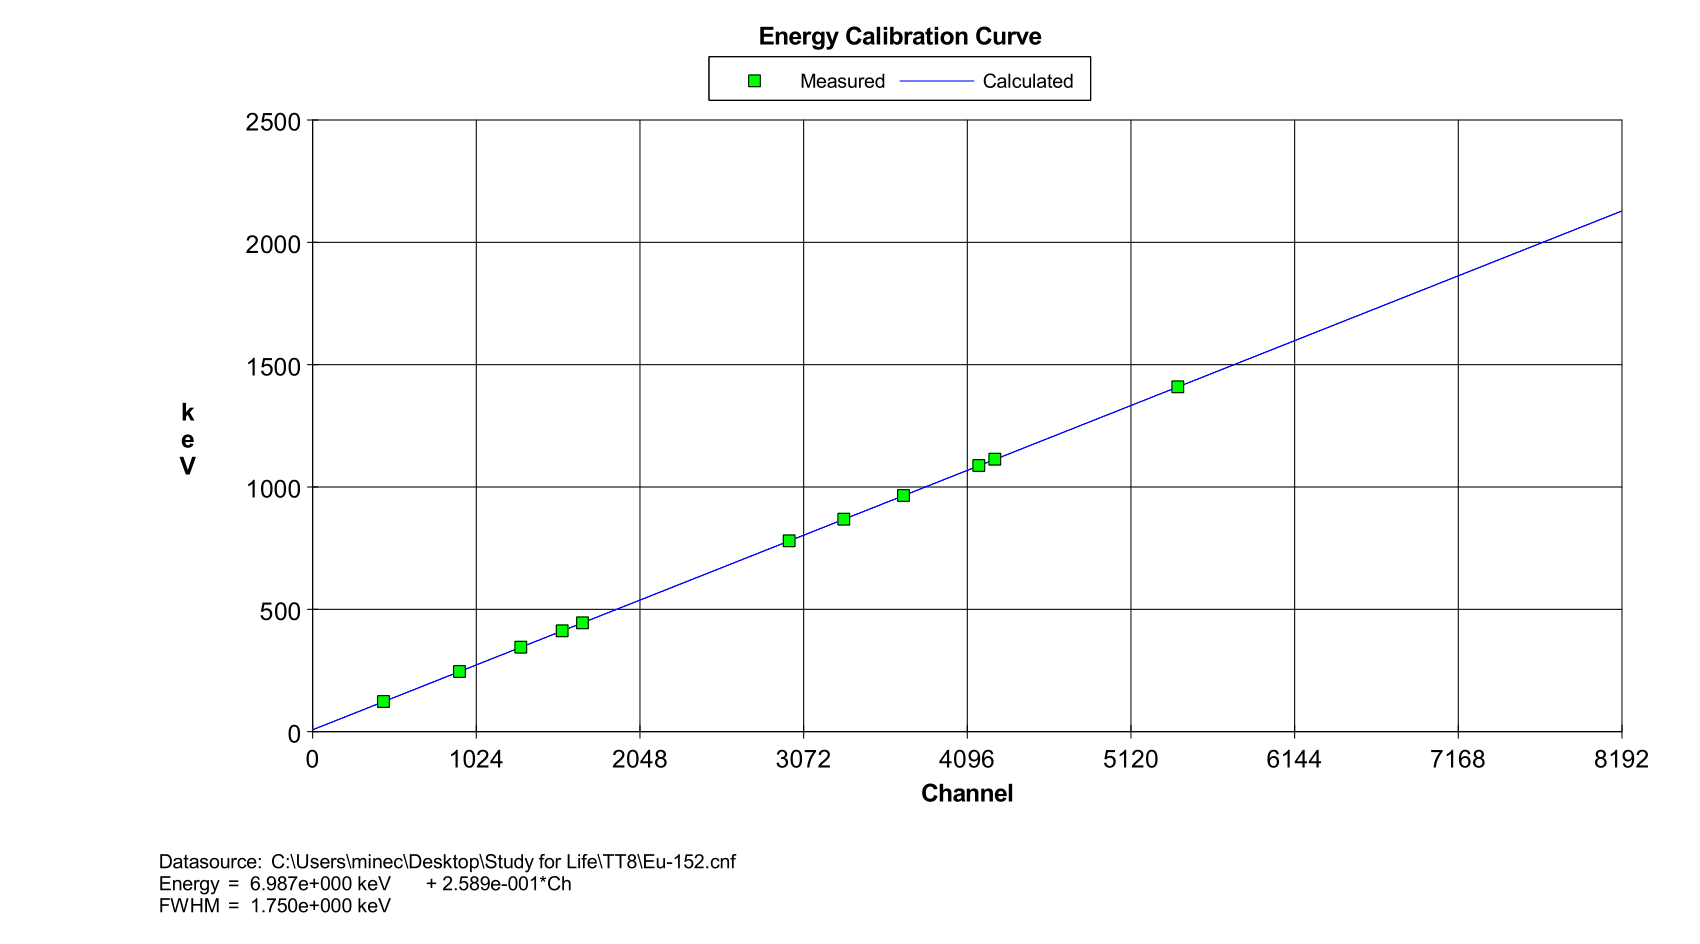
\includegraphics[width=1\linewidth]{peakup}}
\end{figure}
\begin{figure}[ht]
  \centering
  \subfigure[Phương trình chuẩn của Excel]{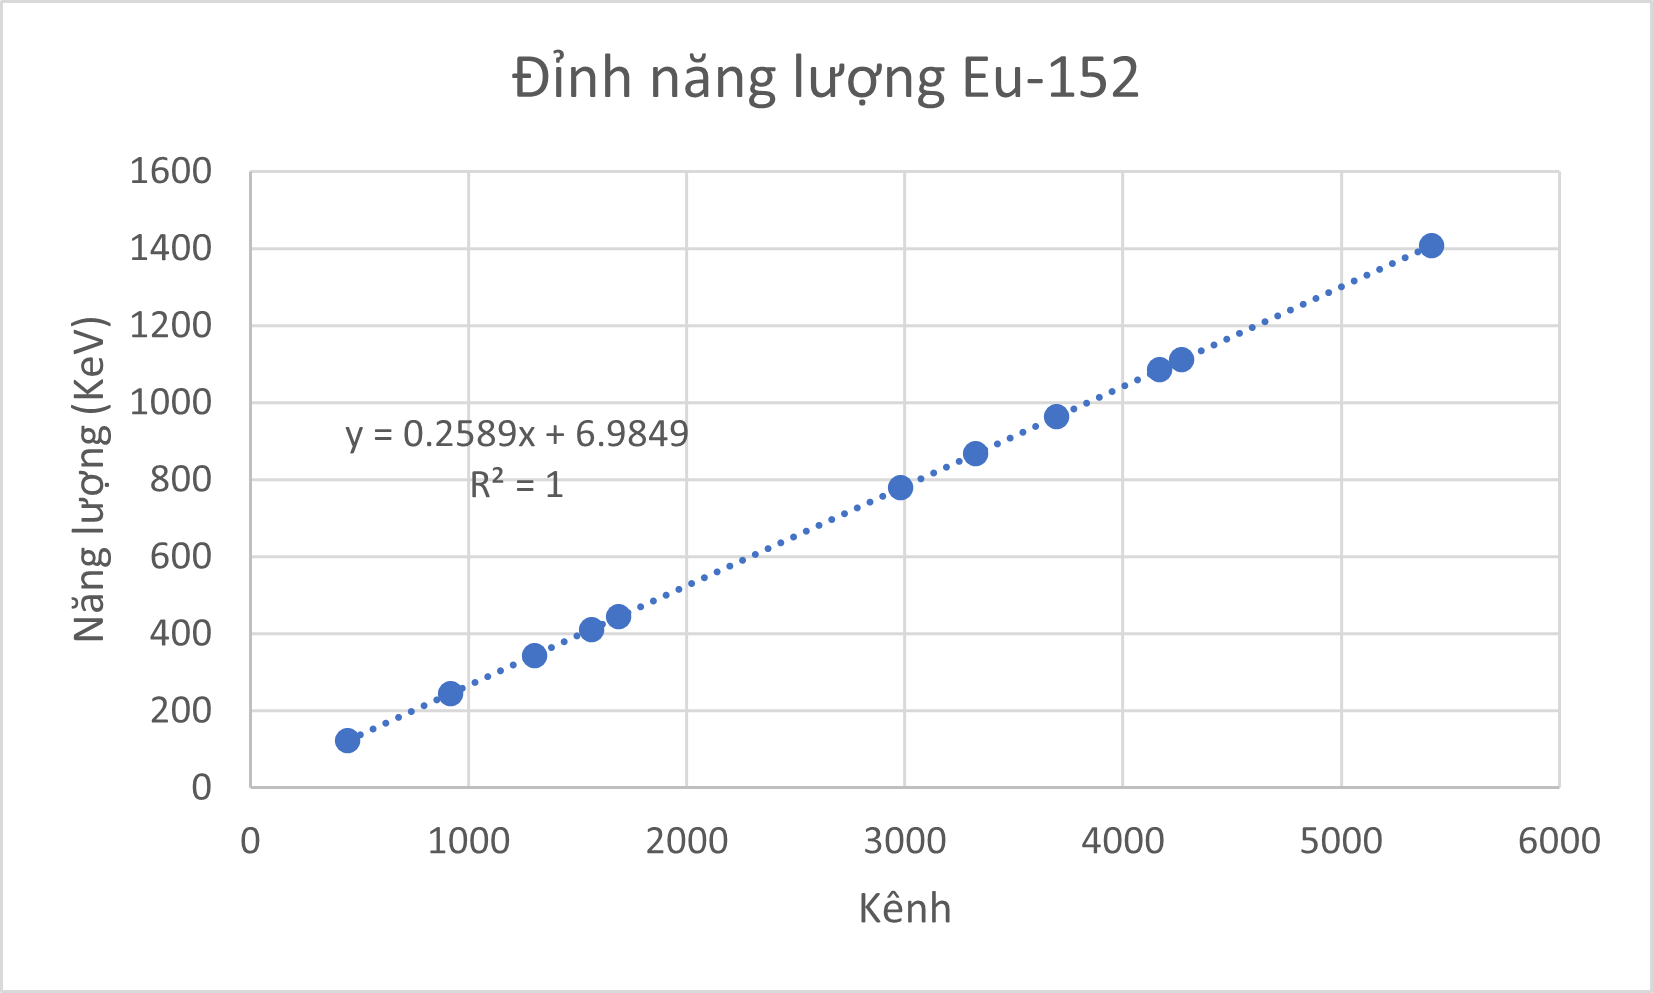
\includegraphics[width=1\linewidth]{PeakEx}}
\end{figure}
%
\newpage
\subsection{Xác định năng lượng và tên đồng vị phóng xạ X}
Từ phương trình (4), ta suy ra được các dãy năng lượng
\begin{table}[!ht]
    \centering
    \resizebox{\columnwidth}{!}{%
    \begin{tabular}{|c|c|c|c|c|c|c|c|c|}
    \hline
        \textbf{Kênh} & 194 & 295 & 1057 & 1173 & 1376 & 1482 & 4573 & 5203 \\ \hline
        \textbf{Năng lượng (KeV)} & 57,21 & 83,36 & 280,64 & 310,67 & 363,23 & 390,67 & 1190,93 & 1354,04 \\ \hline
    \end{tabular}
    }
\end{table} \\
Theo tìm kiếm trên Laraweb thì đây là nguồn ${}^{143}Ce$ có $T_{1/2} = 33,04 \ h$
\begin{table}[!ht]
\centering
\begin{tabular}{cccc}
\hline
Energy (keV) & Intensity (\%) & Type & Origin*  \cr \hline
57,356 (7) & 11,7 (4) & $\gamma$ & Pr-143  \cr
272,9 (2) & 0,0043 (43) & $\gamma$ & Pr-143  \cr
338,3 (2) & 0,0009 (5) & $\gamma$ & Pr-143  \cr
350,619 (3) & 3,23 (4) & $\gamma$ & Pr-143  \cr
389,64 (2) & 0,0364 (18) & $\gamma$ & Pr-143  \cr
1 160,58 (6) & 0,0024 (3) & $\gamma$ & Pr-143  \cr
1 340,1 (1) & 0,00308 (14) & $\gamma$ & Pr-143  \cr \hline
\end{tabular}
\end{table} \\
\vspace{0.25cm}
%
\subsection{Vẽ giá trị thực nghiệm và giá trị làm khớp trên một đồ thị}
\begin{center}
  {\includegraphics[scale=0.75]{nguonX3D}}
\end{center}
%
\newpage
\clearpage\thispagestyle{empty}\addtocounter{page}{-1} 
\clearpage
\mbox{}
\end{document}